\documentclass[12pt,a4paper]{article}
\usepackage{graphicx}
\usepackage{hyperref}
\usepackage{listings}

\title{02.rpc.file.transfer.tex}
\author{Chu Hong Quan}
\date{\}

\begin{document}

\maketitle

\section*{1. RPC service design}
The RPC service was designed using Python's \texttt{xmlrpc.server} module. It includes the following key functionalities:
\begin{itemize}
    \item \texttt{upload}: Allows the client to upload a file to the server.
    \item \texttt{download}: Allows the client to download a file from the server.
    \item \texttt{list}: Lists all files currently available on the server.
\end{itemize}

Below is a high-level architecture diagram of the RPC-based file transfer system:

\begin{center}
    \includegraphics[width=0.8\textwidth]{rpc_architecture.png}
    \captionof{figure}{RPC Service Design Architecture}
\end{center}

\section*{2. System organization}
The system consists of two main components:
\begin{itemize}
    \item \textbf{Server:} Hosts the RPC service and handles file operations like upload, download, and listing.
    \item \textbf{Client:} Connects to the server, invokes RPC methods, and provides user-friendly interaction for file transfers.
\end{itemize}

The system is organized as shown below:

\begin{center}
    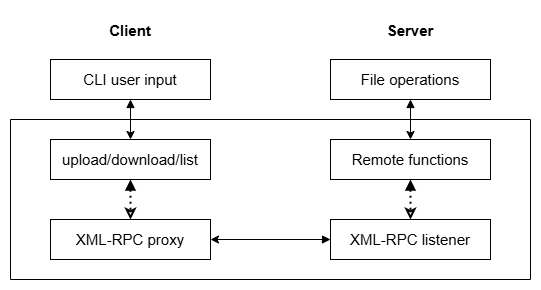
\includegraphics[width=0.8\textwidth]{system_organization.png} % Replace with your organization diagram
    \captionof{figure}{System Organization}
\end{center}

\section*{3. Implementation}
Here are the key code snippets for implementing the file transfer:

\subsection*{Server Code}
\begin{lstlisting}[language=Python, caption=Server Code]
from xmlrpc.server import SimpleXMLRPCServer
import os

def upload_file(file_name, file_data):
    with open(file_name, 'wb') as file:
        file.write(file_data.data)
    return f"File '{file_name}' uploaded successfully."

def download_file(file_name):
    if os.path.exists(file_name):
        with open(file_name, 'rb') as file:
            return file.read()
    else:
        return "ERROR: File not found."

def list_files():
    return os.listdir('.')

def start_server(host='localhost', port=5000):
    server = SimpleXMLRPCServer((host, port), allow_none=True)
    print(f"Server started at {host}:{port}")
    server.register_function(upload_file, "upload")
    server.register_function(download_file, "download")
    server.register_function(list_files, "list")
    server.serve_forever()

if __name__ == '__main__':
    start_server()

\end{lstlisting}

\subsection*{Client Code}
\begin{lstlisting}[language=Python, caption=Client Code]
import xmlrpc.client
import os

def upload_file(client, file_path):
    file_name = os.path.basename(file_path)
    with open(file_path, 'rb') as file:
        file_data = file.read()
    result = client.upload(file_name, file_data)
    print(result)

def download_file(client, file_name, save_as=None):
    file_data = client.download(file_name)
    if isinstance(file_data, bytes):
        save_as = save_as or file_name
        with open(save_as, 'wb') as file:
            file.write(file_data)
        print(f"File '{file_name}' downloaded successfully as '{save_as}'.")
    else:
        print(file_data)

def list_files(client):
    files = client.list()
    print("Files on server:")
    for file in files:
        print(f"- {file}")

if __name__ == '__main__':
    server_address = "http://localhost:5000/"
    client = xmlrpc.client.ServerProxy(server_address)

    while True:
        print("\nOptions:")
        print("1. Upload a file")
        print("2. Download a file")
        print("3. List files on server")
        print("4. Exit")

        choice = input("Enter your choice: ").strip()
        
        if choice == '1':
            file_path = input("Enter the path of the file to upload: ").strip()
            upload_file(client, file_path)
        elif choice == '2':
            file_name = input("Enter the name of the file to download: ").strip()
            save_as = input("Enter the name to save the file locally (leave blank to use original name): ").strip()
            download_file(client, file_name, save_as or None)
        elif choice == '3':
            list_files(client)
        elif choice == '4':
            print("Exiting...")
            break
        else:
            print("Invalid choice. Please try again.")

\end{lstlisting}

\end{document}
